
\begin{frame}{‌کدهای هافمن}
\begin{itemize}\itemr
\item[-]
کدهای هافمن
\fn{1}{Huffman codes}
برای فشرده‌سازی داده‌ها استفاده می‌شوند. این کدها بسته به ویژگی داده‌ها، می‌توانند بین ۲۰ تا ۹۰ درصد در میزان حافظه مورد نیاز برای ذخیره‌سازی داده‌ها صرفه جویی کنند.
\item[-]
 الگوریتم حریصانه هافمن جدولی شامل تعداد تکرار حروف دریافت کرده، سپس برای هر حرف یک کد تولید می‌کند، به طوری که ذخیرهٔ یک متن با استفاده از کدهای تولید شده کمترین میزان حافظه را اشغال کند.
\item[-]
فرض کنید یک فایل داده‌ای داریم که شامل
۱۰۰،۰۰۰
حرف (کاراکتر) است و می‌خواهیم فایل را به صورت فشرده ذخیره کنیم و همچنین می‌دانیم ۶ حرف اول الفبا دارای تعداد تکرارهای ذکر شده در جدول زیر هستند.
\begin{figure}
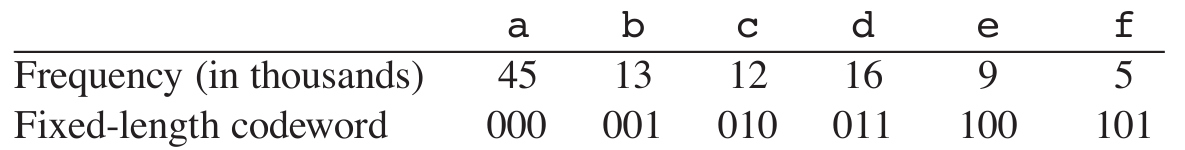
\includegraphics[width=0.7\textwidth]{figs/chap05/huffman-example}
\end{figure}
\end{itemize}
\end{frame}


\begin{frame}{‌کدهای هافمن}
\begin{itemize}\itemr
\item[-]
برای مثال حرف a در این فایل
۴۵،۰۰۰
بار و حرف b تعداد
۱۳،۰۰۰
بار تکرار شده‌اند.
\item[-]
برای نمایش داده‌ها در این فایل راه‌های زیادی وجود دارد. در اینجا از یک کد گذاری دودویی استفاده می‌کنیم. به ازای هر یک از حروف الفبا یک عدد دودویی در نظر گرفته و آن حرف را با کد در نظر گرفته شده نمایش می‌دهیم. به این کدهای دودویی
\fn{1}{binary character  code}
،به اختصار کد می‌گوییم.
\item[-]
می‌توانیم از کدهایی با طول ثابت
\fn{2}{fixed-length code}
استفاده کنیم، که در اینصورت به تعداد
\m{ \lceil \lg n \rceil}
بیت برای نمایش n حرف نیاز داریم. برای ۶ حرف به ۳ بیت نیاز داریم :
\m{a = 000}،
\m{b = 001}،
\m{c = 010}،
\m{d = 011}،
\m{e = 100}و
\m{f = 101}.
\item[-]
با استفاده از این روش کد گذاری برای یک فایل شامل
۱۰۰،۰۰۰
حرف به
۳۰۰،۰۰۰
بیت نیاز داریم. اما آیا می‌توانیم با تعداد کمتری بیت این فایل را ذخیره کنیم؟
\end{itemize}
\end{frame}


\begin{frame}{‌کدهای هافمن}
\begin{itemize}\itemr
\item[-]
برای فشرده‌سازی این فایل متنی و ذخیره‌سازی حروف به طور کارامدتر از کدهایی با طول متغیر
\fn{1}{variable-length code}
استفاده می‌کنیم.
\item[-]
برای نمایش حروفی که تعداد تکرار بیشتری دارند، از کدهای کوتاه‌تر و برای نمایش حروفی که تعداد تکرار کمتری دارند، از کدهای بلندتر استفاده می‌کنیم.
\end{itemize}
\end{frame}


\begin{frame}{‌کدهای هافمن}
\begin{itemize}\itemr
\item[-]
برای مثال یک روش کدگذاری با کدهای طول متغیر در شکل زیر نمایش داده شده است.
\begin{figure}
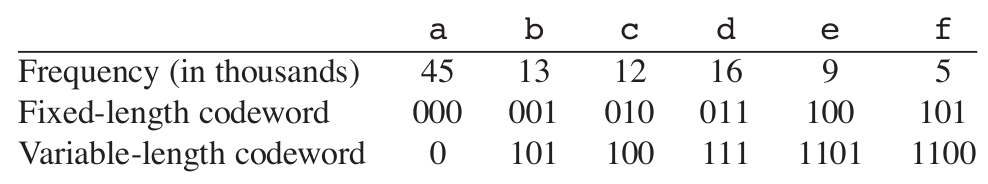
\includegraphics[width=0.7\textwidth]{figs/chap05/huffman-vlc}
\end{figure}
\item[-]
در اینجا از بیت صفر برای نمایش a و عدد چهاربیتی
۱۱۰۰
برای نمایش حروف f استفاده می‌کنیم.
\item[-]
برای نمایش یک فایل شامل
۱۰۰،۰۰۰
حرف با تعداد‌های تکرار ذکر شده به تعداد بیت زیر نیاز داریم‌ :
\begin{align*}
\m{(45 \times 1 + 13 \times 3 + 12 \times 3 + 16 \times 3 + 9 \times 4 + 5 \times 4) \times 1000 = 224000~~\text{bit} }
\end{align*}
\item[-]
بنابراین با استفاده از این روش کدگذاری توانستیم به جای ۳۰۰ هزار بیت از ۲۲۴ هزار بیت استفاده کنیم و حدود ۲۵ درصد در فضای حافظهٔ مورد نیاز صرفه‌جویی کنیم.
\end{itemize}
\end{frame}


\begin{frame}{‌کدهای هافمن}
\begin{itemize}\itemr
\item[-]
در روش کدگذاری استفاده شده، هیچ‌یک از کدها پیشوند کدهای دیگر نبودند. بدین ترتیب به افزودن خط فاصله بین کدها نیازی نداریم و می‌توانیم کدهای یکتا را شناسایی کنیم. به این مجموعهٔ کد، کدهای بدون پیشوند
\fn{1}{prefix-free code}
می‌گوییم.
\item[-]
ثابت شده‌است که کدهای بدون پیشوند بهینه‌ترین روش برای فشرده‌سازی اطلاعات است و هیچ روش کدگذاری بهینه‌تری برای فشرده‌سازی بیشتر وجود ندارد.
\item[-]
با استفاده از روش کدگذاری می‌توانیم کلمهٔ face را به صورت
\begin{align*}
\m{1100 \cdot 0 \cdot 100 \cdot 1101 = 110001001101}
\end{align*}
ذخیره کنیم. در اینجا عملگر
\m{" \cdot "}
به معنی الحاق دو رشته است.
\end{itemize}
\end{frame}


\begin{frame}{‌کدهای هافمن}
\begin{itemize}\itemr
\item[-]
کدهای بدون پیشوند فرایند کدگشایی را ساده می‌کنند. از آنجایی که هیچ کدی پیشوند کد دیگری نیست، کدگذاری یک فایل ابهام ایجاد نمی‌کند. برای کدگشایی یک فایل از ابتدای فایل شروع می‌کنیم و کدها را به ترتیب تبدیل به حروف می‌کنیم.
\item[-]
برای مثال در کدگشایی رشتهٔ
\m{100011001101}
کد
\m{1}
یا
\m{10}
یا
\m{1000}
وجود ندارند و تنها کدی که می‌توان در ابتدای این رشته تشخیص داد، کد
\m{100}
است. این کد معادل کلمه
cafe
می‌باشد.
\begin{align*}
\m{100011001101 = 100 \cdot 0 \cdot 1100 \cdot 1101 = cafe}
\end{align*}
\begin{figure}
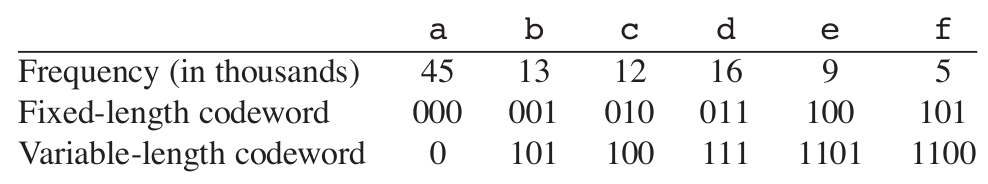
\includegraphics[width=0.7\textwidth]{figs/chap05/huffman-vlc}
\end{figure}
\end{itemize}
\end{frame}


\begin{frame}{‌کدهای هافمن}
\begin{itemize}\itemr
\item[-]
در فرایند کدگشایی برای جستجوی بهینهٔ کدها و حروف متناظر آنها از یک درخت دودویی استفاده می‌کنیم. برگ‌های این درخت دودویی، حروف متناظر با کدهایی هستند که از الحاق کدهای روی یال‌ها از ریشه تا برگ مورد نظر به دست می‌آیند.
\item[-]
به عبارت دیگر کد مربوط به یک حرف درواقع یک مسیر از ریشه تا حرف مورد نظر است به طوری‌که صفر به معنای رفتن به سمت فرزند سمت چپ و یک به معنای رفتن به فرزند سمت راست است.
\end{itemize}
\end{frame}


\begin{frame}{‌کدهای هافمن}
\begin{itemize}\itemr
\item[-]
شکل‌های زیر دو درخت متفاوت برای کدگذاری حروف را نشان می‌دهند.
\begin{figure}
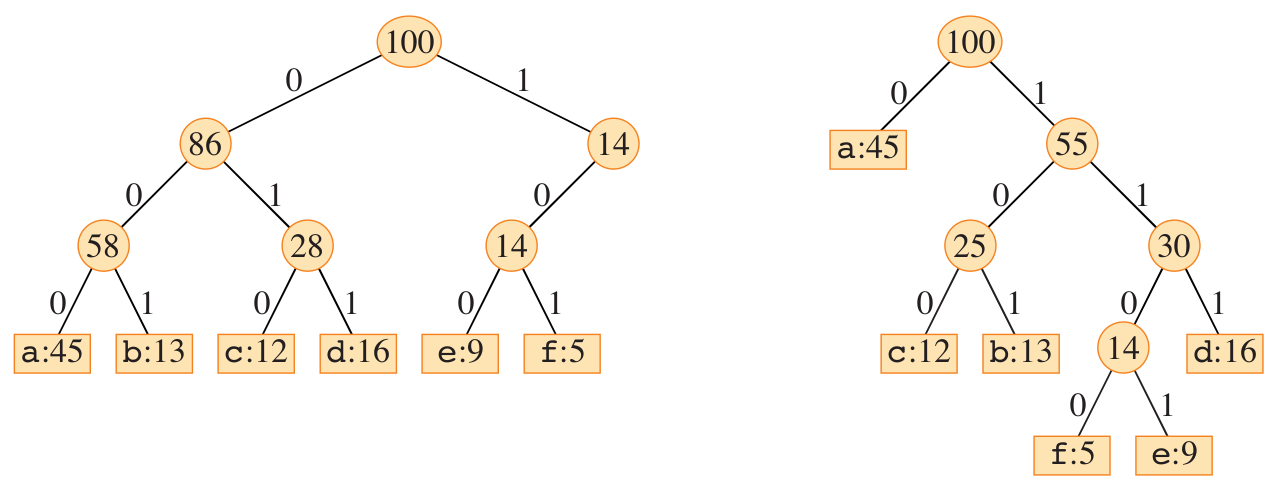
\includegraphics[width=0.9\textwidth]{figs/chap05/huffman-tree}
\end{figure}
\end{itemize}
\end{frame}


\begin{frame}{‌کدهای هافمن}
\begin{itemize}\itemr
\item[-]
می‌توان ثابت کرد که یک کدگذاری بهینه همیشه توسط یک درخت دودویی پُر
\fn{1}{full binary tree}
(درخت اکیدا دودویی)
نشان داده می‌شود،
بدین معنی که هر رأس میانی در درخت بهینه الزاما دارای دو فرزند است. در شکل زیر در سمت چپ، درخت دودویی پر نیست، زیرا به ازای کد ۱۱ هیچ حرفی وجود ندارد،
پس کدگذاری توسط این درخت نمی‌تواند یک کدگذاری بهینه باشد،
 اما درخت سمت راست یک درخت دودویی پر را نشان می‌دهد.
\begin{figure}
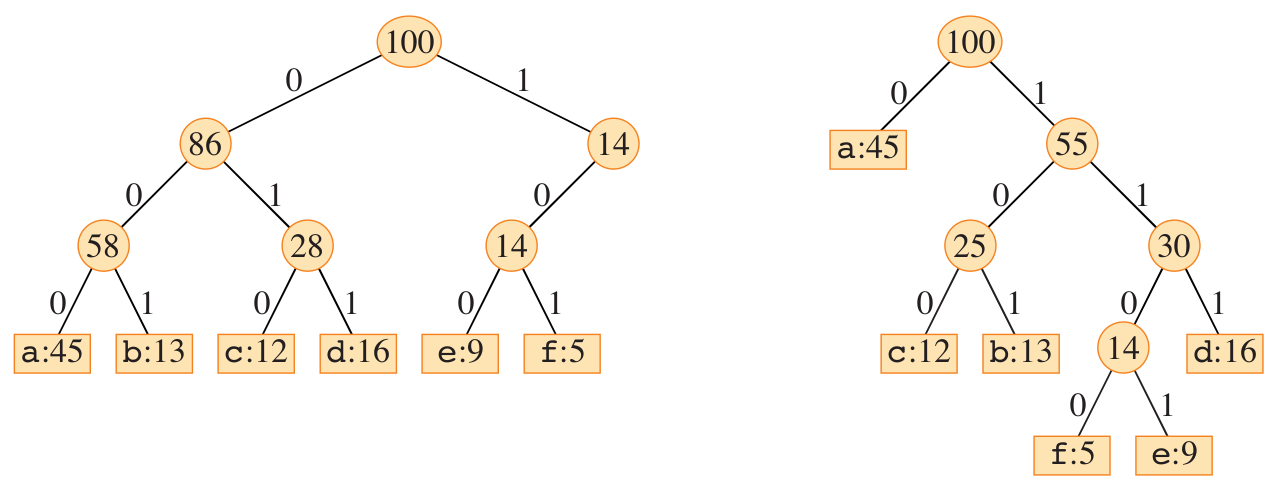
\includegraphics[width=0.6\textwidth]{figs/chap05/huffman-tree}
\end{figure}
%\item[-]
%در درخت سمت چپ از کد ۱ برای هیچ حرفی استفاده نشده است و به همین دلیل این کدگذاری نمی‌تواند بهینه باشد.
\end{itemize}
\end{frame}


\begin{frame}{‌کدهای هافمن}
\begin{itemize}\itemr
\item[-]
یک درخت دودویی پر با 
\m{n}
 برگ الزاما 
\m{n-1}
رأس غیربرگ دارد.
\item[-]
اگر
\m{C}
الفبای مورد نظر برای کدگذاری باشد، درختی که برای کدهای بدون پیشوند بهینه به دست می‌آید، دارای
\m{|C|}
برگ است که هر برگ متناظر با یک حرف است و تعداد
\m{|C| - 1}
رأس میانی (غیربرگ) در درخت داریم.
\end{itemize}
\end{frame}


\begin{frame}{‌کدهای هافمن}
\begin{itemize}\itemr
\item[-]
اگر درخت
\m{T}
درختی برای کدهای بدون پیشوند باشد، می‌توانیم تعداد بیت‌های مورد نیاز برای کدگذاری یک فایل را محاسبه کنیم. به ازای هر حرف c در الفبای
\m{C}
 ، فرض کنید
\m{c.freq}
تعداد تکرار آن حرف در فایل باشد و فرض کنید
\m{d_T(c)}
عمق برگ متناظر با حرف c در درخت باشد. دقت کنید که
\m{d_T(c)}
طول کد متناظر با حرف c نیز هست. در اینصورت تعداد بیت‌های مورد نیاز برای کدگذاری فایل داده‌ای برابراست با
\begin{align*}
\m{B(T) = \sum_{c \in C} c.freq \times d_T(c)}
\end{align*}
\item[-]
به مقدار
\m{B(T)}
هزینه
\fn{1}{cost}
درخت T می‌گوییم.
\end{itemize}
\end{frame}


\begin{frame}{‌کدهای هافمن}
\begin{itemize}\itemr
\item[-]
هافمن یک الگوریتم حریصانه ابداع کرد که کدهای بدون پیشوند بهینه تولید می‌کند. این کدها به کدهای هافمن مشهور هستند.
%\item[-]
%ابتدا الگوریتم حریصانهٔ تولید کدهای هافمن را توضیح می‌دهیم و سپس اثبات می‌کنیم چرا الگوریتم حریصانه در اینجا می‌تواند مورد استفاده قرار بگیرد.
\item[-]
ورودی الگوریتم هافمن مجموعهٔ
\m{C}
شامل n حرف است، به طوری که هر عضو
\m{c \in C}
یک حرف است که ویژگی
\m{c.freq}
تعداد تکرار آن را نشان می‌دهد.
\item[-]
این الگوریتم درخت T را برای تولید کدهای بهینه می‌سازد. این درخت از پایین به بالا تولید می‌شود، بدین معنی که الگوریتم با
\m{|C|}
برگ آغاز می‌کند و با ادغام این برگ‌ها به صورت ساختار درختی، کل درخت را تا ریشه می‌سازد.
\item[-]
در این الگوریتم از یک صف اولویت استفاده می‌شود که حروف با کمترین تعداد‌های تکرار به ترتیب از صف خارج می‌شوند.
\end{itemize}
\end{frame}


\begin{frame}{‌کدهای هافمن}
\begin{itemize}\itemr
\item[-]
الگوریتم هافمن به صورت زیر است.
\begin{algorithm}[H]\alglr
  \caption{Huffman} 
  \begin{algorithmic}[1]
   \Func{Huffman}{C}
   \State n = |C|
   \State Q = C
   \For{i = 1 \To n - 1}
   			\State allocate a new node z
   			\State x = Extract-Min(Q)
   			\State y = Extract-Min(Q)
   			\State z.left = x
   			\State z.right = y
   			\State z.freq = x.freq + y.freq
   			\State Insert(Q,z)
   	\EndFor
   	\State \Return Extract-Min(Q) \LeftComment{the root of the tree is the only node left}                       
  \end{algorithmic}
  \label{alg:merge}
\end{algorithm}
\end{itemize}
\end{frame}


\begin{frame}{‌کدهای هافمن}
\begin{itemize}\itemr
\item[-]
برای مثالی که در قبل مطرح کردیم، الگوریتم هافمن به صورت زیر عمل می‌کند.
\begin{figure}
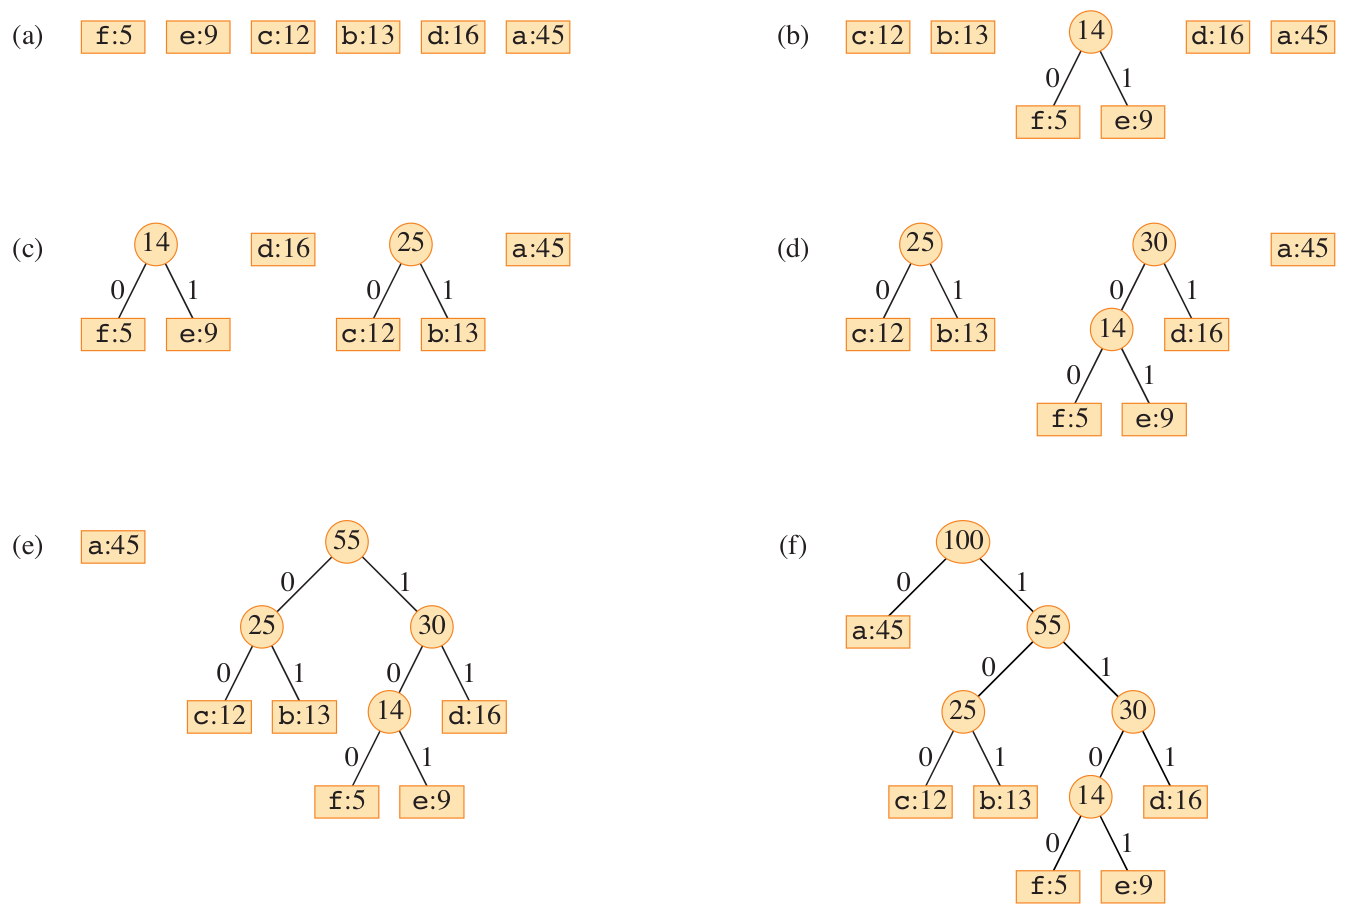
\includegraphics[width=0.7\textwidth]{figs/chap05/huffman-alg-ex}
\end{figure}
\end{itemize}
\end{frame}


\begin{frame}{‌کدهای هافمن}
\begin{itemize}\itemr
\item[-]
زمان الگوریتم هافمن به نحوهٔ پیاده‌سازی صف اولویت بستگی دارد. فرض کنیم با بهینه‌ترین الگوریتم موجود، صف اولویت برای یک الفبا با n حرف در زمان
\m{O(n)}
ساخته می‌شود.
\item[-]
حلقهٔ اصلی در الگوریتم هافمن
\m{n-1}
بار تکرار می‌شود، زیرا تعداد رئوس غیربرگ
\m{n-1}
است
 و از آنجایی که در هر بار استفاده از صف اولویت به زمان
\m{\lg n}
نیاز داریم، بنابراین زمان اجرای الگوریتم
\m{O(n \lg n)}
است.
\item[-]
بنابراین کل زمان اجرای الگوریتم هافمن برای الفبای n حرفی برابراست با
\m{O(n \lg n)}.
\end{itemize}
\end{frame}


\begin{frame}{‌کدهای هافمن}
\begin{itemize}\itemr
\item[-]
برای اثبات اینکه الگوریتم حریصانه هافمن درست است، نشان می‌دهیم مسئله تعیین کدهای بدون پیشوند بهینه دارای ویژگی انتخاب حریصانه است.
\item[-]
به عبارت دیگر می‌خواهیم اثبات کنیم دو رأس با کمترین تعداد تکرار الزاما در درخت کدهای بهینه همزاد یکدیگرند و در بیشترین عمق قرار می‌گیرند.
\end{itemize}
\end{frame}


\begin{frame}{‌کدهای هافمن}
\begin{itemize}\itemr
\item[-]
قضیه : فرض کنید
\m{C}
یک الفبا باشد به طوری‌که
\m{c \in C}
دارای تعداد تکرار
\m{c.freq}
باشد. فرض کنید x و y دو حرف در C با کمترین تعداد‌های تکرار باشند. آنگاه یک کدگذاری بدون پیشوند بهینه برای C وجود دارد به طوری‌که x و y طول یکسانی دارند و تنها در بیت آخر متفات‌اند، یعنی همزاد یکدیگرند و همچنین در بیشترین عمق درخت قرار دارند.
\end{itemize}
\end{frame}


\begin{frame}{‌کدهای هافمن}
\begin{itemize}\itemr
\item[-]
اثبات : ایدهٔ اثبات این است که درخت
\m{T}
که یک درخت بهینهٔ بدون پیشوند را در نظر بگیریم و آن را تغییر دهیم تا یک درخت دودویی بدون پیشوند دیگر ساخته شود به طوری‌که در درخت ساخته شده x و y همزاد
\fn{1}{sibiling}
و در عمق بیشینه در درخت
\m{T}
باشند. چنین درختی که در آن x و y همزاد یکدیگرند یعنی طول یکسان دارند و تنها در بیت آخر متفاوت‌اند، نیز یک درخت بهینه خواهد بود.
\item[-]
فرض کنید a و b دو حرف باشند که در درخت
\m{T}
همزاد هستند و در بیشترین عمق درخت قرار دارند. حال فرض کنید
\m{a.freq \leqslant b.freq}
و
\m{x.freq \leqslant y.freq}.
از آنجایی‌که
\m{x.freq}
و
\m{y.freq}
کمترین تعداد‌های تکرار هستند و
\m{a.freq}
و
\m{b.freq}
دو تعداد تکرار دلخواه هستند، بنابراین خواهیم داشت
\m{x.freq \leqslant a.freq}
و
\m{y.freq \leqslant b.freq}.
\item[-]
بنابراین می‌توانیم داشته باشیم
\m{x.freq = a.freq}
و
\m{y.freq = b.freq}
که در اینصورت قضیه به طور بدیهی درست است، زیرا a و b دارای کمترین تعداد تکرار هستند.
 پس فرض می‌کنیم تعداد تکرارهای
 x 
 و
 y
 متفاوت از a و b هستند.
\end{itemize}
\end{frame}


\begin{frame}{‌کدهای هافمن}
\begin{itemize}\itemr
\item[-]
همانطور که شکل زیر نشان می‌دهد، فرض کنید جای a و x را در درخت
\m{T}
عوض می‌کنیم و درخت
\m{T'}
را به‌دست می‌آوریم و جای b و y را در درخت 
\m{T'}
عوض کرده،
درخت
\m{T''}
را به دست می‌آوریم.
\begin{figure}
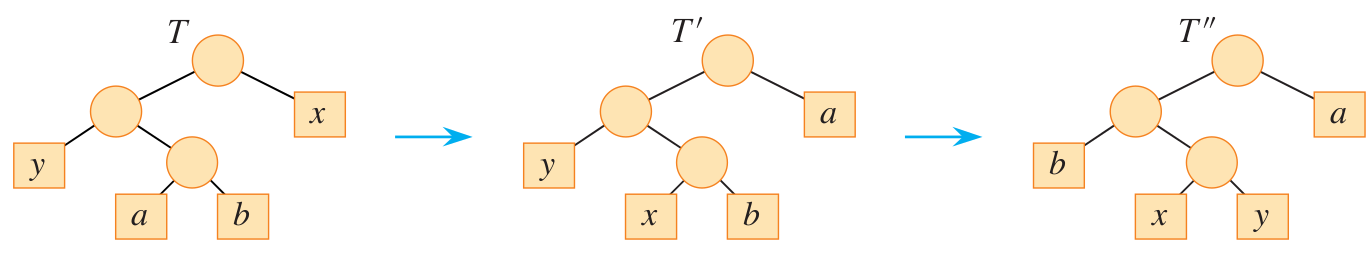
\includegraphics[width=0.9\textwidth]{figs/chap05/huffman-proof}
\end{figure}
\item[-]
نشان می‌دهیم که هزینهٔ درخت
\m{T''}
کوچکتر یا مساوی درخت
\m{T}
 است.
 از آنجایی که فرض کردیم درخت 
 \m{T}
 یک درخت بهینه است، بنابراین هزینه درخت 
 \m{T''}
 و
\m{T}
باید برابر باشد.
\end{itemize}
\end{frame}


\begin{frame}{‌کدهای هافمن}
\begin{itemize}\itemr
\item[-]
تفاوت هزینهٔ درخت
\m{T}
و
\m{T'}
به صورت زیر خواهد بود.
\begin{align*}
\m{B(T)} & \m{- B(T')}\\
&\m{= \sum_{c \in C} c.freq \cdot d_T(c) - \sum_{c \in C} c.freq \cdot d_{T'}(c)}\\
&\m{= x.freq \cdot d_T(x) + a.freq \cdot d_T(a) - x.freq \cdot d_{T'}(x) - a.freq \cdot d_{T'}(a)}\\
&\m{= x.freq \cdot d_T(x) + a.freq \cdot d_T(a) - x.freq \cdot d_T(a) - a.freq \cdot d_T(x)}\\
&\m{= (a.freq - x.freq) (d_T(a) - d_T(x))}\\
&\m{\geqslant 0}
\end{align*}
\end{itemize}
\end{frame}


\begin{frame}{‌کدهای هافمن}
\begin{itemize}\itemr
\item[-]
از آنجایی که
\m{a.freq - x.freq}
و همچنین
\m{d_T(a) - d_T(x)}
غیر منفی هستند، بنابراین مقدار
\m{B(T) - B(T')}
مثبت است.
\item[-]
درواقع
\m{a.freq - x.freq}
غیر منفی است زیرا x یک برگ با حداقل تعداد تکرار است و
\m{d_T(a) - d_T(x)}
غیر منفی است زیرا a یک برگ با عمق بیشینه در درخت
\m{T}
است.
\item[-]
به همین ترتیب تعویض y و b هزینه را افزایش نمی‌دهد و بنابراین
\m{B(T') - B(T'')}
نیز غیر منفی است.
\item[-]
بنابراین
\m{B(T'') \leqslant B(T') \leqslant B(T)}
و چون
\m{T}
بهینه است بنابراین داریم
\m{B(T) \leqslant B(T'')}
و بنابراین
\m{B(T'') = B(T)}
در نتیجه
\m{T''}
یک درخت بهینه است که در آن x و y دو برگ همزاد با عمق حداکثر هستند و قضیه ثابت می‌شود.
\end{itemize}
\end{frame}


\begin{frame}{‌کدهای هافمن}
\begin{itemize}\itemr
\item[-]
این قضیه در واقع نشان می‌دهد که ساختن درخت بهینه، می‌تواند با انتخاب حریصانه ادغام دو حرف با کمترین تعداد تکرار آغاز شود و ادامه یابد. بنابراین از بین همهٔ انتخاب‌ها برای ادغام الگوریتم هافمن دو حرف با کمترین تعداد را در هر مرحله انتخاب می‌کند که یک انتخاب بهینه است، و همچنین درخت کلی به دست آمده در نهایت یک درخت بهینه خوهد بود.
\end{itemize}
\end{frame}


\begin{frame}{‌کدهای هافمن}
\begin{itemize}\itemr
\item[-]
حال می‌خواهیم ثابت کنیم ساختن کدهای بدون پیشوند بهینه دارای ویژگی زیر ساختار بهینه است.
\item[-]
به عبارت دیگر، می‌خواهیم اثبات کنیم اگر رأس z به عنوان پدر رئوس x و y با کمترین تعداد تکرار به همراه بقیه رئوس درخت به جز x و y ، یک درخت کدهای بهینه را تشکیل دهند، آنگاه درختی که در آن x و y به عنوان فرزندان z اضافه شده‌اند نیز درخت کدهای بهینه است.
\end{itemize}
\end{frame}


\begin{frame}{‌کدهای هافمن}
\begin{itemize}\itemr
\item[-]
قضیه : فرض کنید
\m{C}
یک الفبا باشد به طوری‌که برای هر حرف
\m{c \in C}
تعداد تکرار c برابر با
\m{c.freq}
باشد. فرض کنید x و y دو حرف در
\m{C}
با تعداد تکرار حداقل باشند. فرض کنید
\m{C'}
همان الفبای 
\m{C}
 باشد به طوری‌که حروف x و y حذف شده و حرف z به آن اضافه شده است، بنابراین
\m{C' = (C - \{x,y\}) \cup \{z\}}
تعداد تکرار همهٔ حروف در
\m{C'}
برابر با حروف
\m{C}
هستند و همچنین
\m{z.freq = x.freq + y.freq}.
فرض کنید
\m{T'}
درختی باشد که کدهای بدون پیشوند بهینه
\m{C'}
را نمایش می‌دهد. آنگاه درخت
\m{T}
که از درخت
\m{T'}
به دست آمده و در آن رأس z با یک رأس میانی با دو فرزند x و y به جایگزین شده است، کدهای بدون پیشوند بهینه برای الفبای
\m{C}
را نمایش می‌دهد.
\end{itemize}
\end{frame}


\begin{frame}{‌کدهای هافمن}
\begin{itemize}\itemr
\item[-]
اثبات : ابتدا نشان می‌دهیم چگونه هزینه
\m{B(T)}
از درخت
\m{T}
بر اساس هزینهٔ
\m{B(T')}
از درخت
\m{T'}
بیان می‌شود.
\item[-]
به ازای هر حرف
\m{c \in C - \{x,y\}}
، داریم
\m{d_T(c) = d_{T'}(c)}
و بنابراین
\m{c.freq \times d_T(c) = c.freq \times d_{T'}(c)} .
\item[-]
چون
\m{d_T(x) = d_T(y) = d_{T'}(z) + 1}
،بنابراین داریم :
\begin{align*}
\m{x.freq \times d_T(x) + y.fraq \times d_T(y)} & \m{= (x.freq + y.freq)(d_{T'}(z) + 1)}\\
& \m{= z.freq \times d_{T'}(z) + (x.freq + y.freq)}
\end{align*}
\item[-]
بنابراین نتیجه می‌گیریم
\m{B(T) = B(T') + x.freq + y.freq}
که برابر است با
\m{B(T') = B(T) - x.freq - y.freq}.
\item[-]
حال از برهان خلف استفاده می‌کنیم.
\end{itemize}
\end{frame}


\begin{frame}{‌کدهای هافمن}
\begin{itemize}\itemr
\item[-]
فرض کنید
\m{T}
درخت بهینه بدون پیشوند برای
\m{C}
نیست. بنابراین یک درخت
\m{T''}
بهینه وجود دارد به طوری‌که
\m{B(T'') < B(T)}.
درخت
\m{T''}
دو رأس x و y را به عنوان همزاد درخود دارد.
\item[-]
حال فرض کنید
\m{T'''}
همان درخت
\m{T''}
باشد که در آن پدر مشترک x و y با رأس برگ z جایگزین شده است به طوری‌که
\m{z.freq = x.freq + y.freq}
\item[-]
بنابراین :
\begin{align*}
\m{B(T''')} & \m{= B(T'') - x.freq - y.freq}\\
& \m{< B(T) - x.freq - y.freq}\\
& \m{= B(T')}
\end{align*}
\item[-]
به این نتیجه رسیدیم که 
\m{T'''}
یک درخت بهینه برای 
\m{C'}
است، اما با این نتیجه 
 به تناقض می‌رسیم زیرا فرض کردیم
\m{T'}
درخت بدون پیشوند بهینه برای
\m{C'}
است. بنابراین
\m{T}
باید کدهای بدون پیشوند بهینه برای الفبای
\m{C}
را نمایش دهد.
\end{itemize}
\end{frame}


\begin{frame}{‌کدهای هافمن}
\begin{itemize}\itemr
\item[-]
دو قضیهٔ اثبات شده نشان می‌دهند الگوریتم هافمن کدهای بدون پیشوند بهینه تولید می‌کند.
\end{itemize}
\end{frame}
